\FloatBarrier
A simulação para o modelo de \textit{trapping-detrapping} explicado na Seção \ref{sec:trap-detrap-gas-cc} com concentração da superfície dada pela condição de nitretação gasosa, utilizou os parâmetros mencionados na Seção \ref{params_sub}, os parâmetros para nitretação a gás da Seção \ref{sec:param-gas}, temperatura de 673K e os seguinte valores para a aplicação do método numérico:$\Delta t$ e $\Delta x$ utilizados foram 0,0001s e 0,1 $\mu m$, para um tempo total de 8 horas e 20 $\mu m$ de profundidade.

Os resultados dessa simulação estão representados nas Figuras \ref{fig:td-csvar-gas}, \ref{fig:td-csvar-gas-exp} e \ref{fig:td-csvar-gas-both}, as duas primeiras mostram o desenvolvimento do perfil de concentração de nitrogênio no tempo e a última mostra a evolução do perfil de concentração de nitrogênio livre, aprisionado e total .

Na Figura \ref{fig:td-csvar-gas-exp} está também representada os dados experimentais do artigo \cite{christiansen2008nitrogen}. No artigo, o experimento foi realizado com aço AISI 316,  à 440°C, durante 23 horas, com potencial de nitretação de 1,41 $bar^{-1/2}$. 

\begin{figure}[ht]
\centering
	\caption{Resultado simulação para o modelo de \textit{trapping-detrapping} para nitretação gasosa, até 2 horas}
	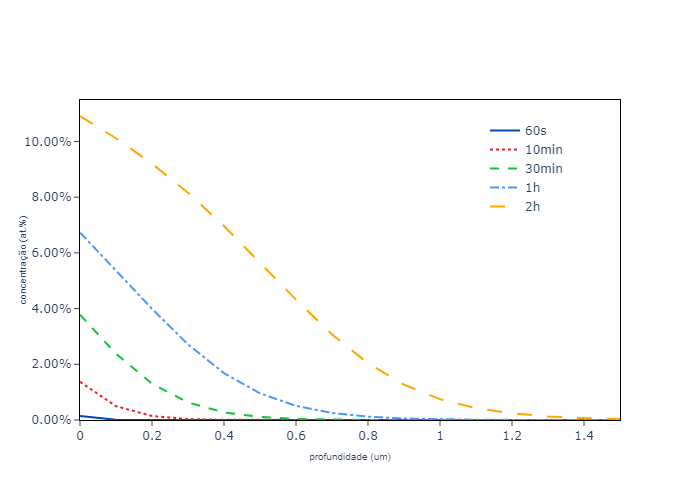
\includegraphics[width=1.0\textwidth]{plot_TrapDetrapGas_zoom}
	\label{fig:td-csvar-gas}
	\centering
	\fonte{Elaborado pela autora}
\end{figure}

\begin{figure}[ht]
\centering
	\caption{Resultado simulação para o modelo de \textit{trapping-detrapping} para nitretação gasosa, até 8 horas, com resultado experimental de \cite{christiansen2008nitrogen}}
	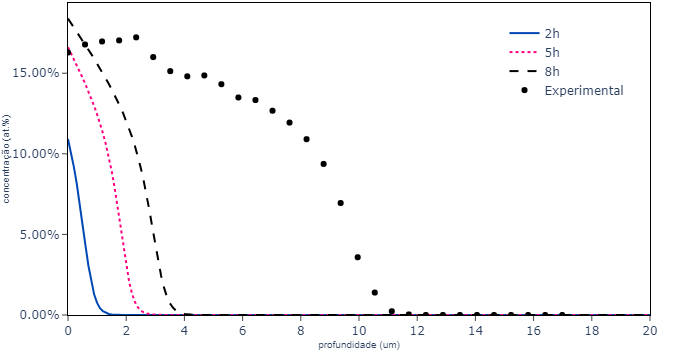
\includegraphics[width=1.0\textwidth]{plot_TrapDetrapGas2Exp}
	\label{fig:td-csvar-gas-exp}
	\centering
	\fonte{Elaborado pela autora}
\end{figure}


\begin{figure}[ht]
\centering
	\caption{Resultado simulação para o modelo de \textit{trapping-detrapping} para nitreação gasosa - Perfil de Concentração de nitrogênio Livre e Aprisionado ao longo do tempo}
	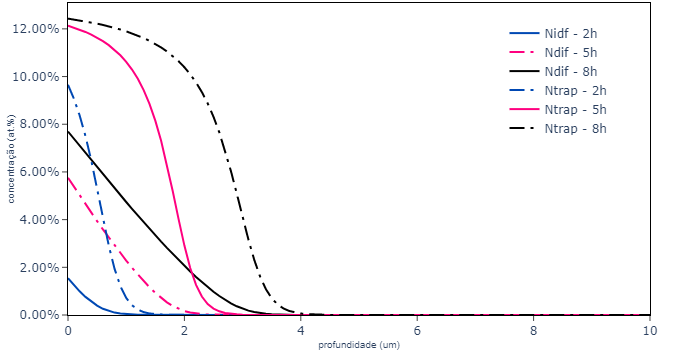
\includegraphics[width=1.0\textwidth]{plot_TrapDetrapGas_analysis}
	\label{fig:td-csvar-gas-both}
	\centering
	\fonte{Elaborado pela autora}
\end{figure}

Na Figura \ref{fig:td-csvar-gas-compara}, foram plotadas ambas as soluções dos dois modelos estudados, para nitretação gasosa, mostrando o perfil de concentração de nitrogênio após 2 horas obtido para cada um.

\begin{figure}[ht]
\centering
	\caption{Resultado da simulação para os dois modelos considerando nitretação gasosa, após 2 horas }
	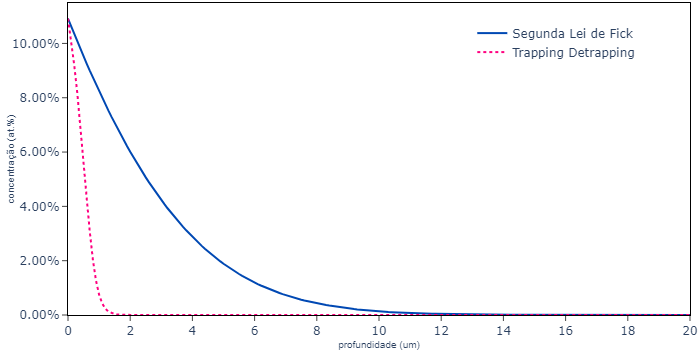
\includegraphics[width=1.0\textwidth]{plot_AmbosGas2h}
	\label{fig:td-csvar-gas-compara}
	\centering
	\fonte{Elaborado pela autora}
\end{figure}
\FloatBarrier